% Chapter Template

\chapter{Feature Extraction} % Main chapter title
\label{Feature Extraction} % Change X to a consecutive number; for referencing this chapter elsewhere, use \ref{ChapterX}
\lhead{Chapter 4. \emph{Feature Extraction}} % Change X to a consecutive number; this is for the header on each page - perhaps a shortened title
Feature extraction is a special form of dimensionality reduction, without loosing important information of data set. When we talk about images or text data generally actual data set is too huge to be processed. We need to use some transformation to extract out some interesting points from the data. Such points should help us in achieving our goal, which can vary from image classification to topic finding anything. Such reduced set of instrumental information is called as set of features. The process of computing these features is called as Feature Vector Extraction. These feature vectors are constructed in a way that they perform the task using reduced representation. 
For the feature extraction from our image data-set augmented with social meta-data, we break the process in two parts:
\begin{itemize}
\item Image Content Based Feature Extraction
\item Social Content Based Feature Extraction
\end{itemize}
In the following part of chapter, we will explain about the features we have used and methodology used for extraction of those features.

%----------------------------------------------------------------------------------------
%	SECTION 1
%----------------------------------------------------------------------------------------

\section{Image Content Based Feature Extraction}
Feature extraction is an important step in image processing. The performance of a classifier depends on the feature vector. Several kind of features are proposed in image processing field. Some primarily used common features for image classification are Color Histogram, HoG, LBP, SIFT, SURF, GLCM etc. Even after extracting important feature vectors, we face the problem of high dimensionality. So for reducing the dimesnionality, we use several other dimesionality reduction techniques. Some important techniques are PCA, Bag-of-words etc. In our work,  we used following visual features:
\begin{itemize}
\item SIFT Features
\item GIST Features
\item COLOR Space Features
\item Texture/GLCM Features
\item HOG-LBP Features
\end{itemize}
In case of HoG-LBP and SIFT features we also used PCA and Bag-of-words model for further dimesnionality reduction. In the following part of this section, we will explain about these features and methodology used for extraction.
\subsection{SIFT Features}
SIFT(Scale-Invariant Feature Transform), as the name suggest, it is a feature descriptor, which is invariant to image scaling. But It is just not only consistent with the variation in scaling, it is also consistent with translation, rotation and till some extent also remains unaffected of (some) variations of the illuminations , 3D projections and other viewing conditions. The SIFT is normally bundled with a feature detector and a feature descriptor. The detector extracts attributed regions from in such a way, that the description of these regions(descriptors) is consistent with all the aforementioned changes (illumination, view point etc). The descriptor associates with the regions a signature which recognize their appearances efficiently and accurately. For example, some sift descriptors are shown in Figure  \ref{fig:siftExample}.
 %%%%%%%%%%%%%%%
 \begin{center}
\begin{figure}
\centering
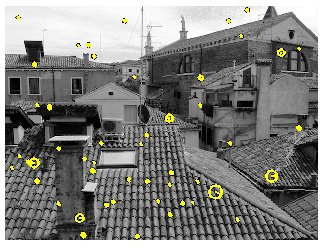
\includegraphics[width=4.5cm, height=4.5cm]{./Pictures/SIFT/siftDescriptorExample.jpg}
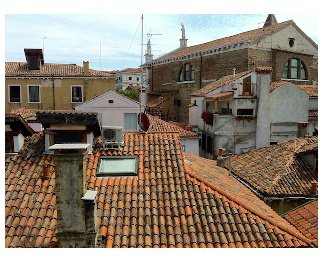
\includegraphics[width=4.5cm, height=4.5cm]{./Pictures/SIFT/siftExample.jpg}
\caption{Example of SIFT Descriptors}
\label{fig:siftExample}
\end{figure}
\end{center}
%%%%%%%%%%%%%%%%
By above-mentioned description, we can easily judge that SIFT features are very instrumental for finding objects and recognizing scenes in an image. SIFT descriptors were first introduced by Lowe \cite{lowe} in ICCV 1999. He took the idea from the primate vision process. The SIFT Features are actually similar to the neurons in inferior temporal cortex of a primate. Features are efficiently extracted through a staged filtering approach that focuses on some key invariable points in scale space. The steps of this filtering approach as mentioned below in Figure \ref{fig:siftProcess}.
 %%%%%%%%%%%%%%%
 \begin{center}
\begin{figure}
\centering
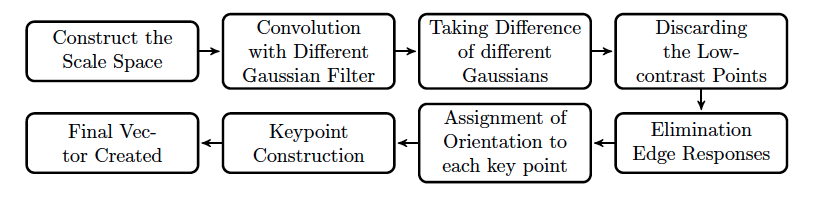
\includegraphics[width=\linewidth]{./Pictures/SIFT/siftSteps.jpg}
\caption{Process Flow of SIFT Descriptor }
\label{fig:siftProcess}
\end{figure}
\end{center}
%%%%%%%%%%%%%%%%
\hspace*{1 cm} SIFT features have been proven very useful in objectives like: natural scene recognition by Li Fei-Fei and Pietro Perona in their paper \cite{naturalSceneRecognition}. It is also very instrumental in object recognition as shown in \cite{lowe}. Motivated by the excellent performance of SIFT Features in Image Categorization, we decide SIFT as one of our features for image classification.\\
    In \cite{naturalSceneRecognition}, Fei fei et al. has shown that dense local scale-variant features performs better compared to sparse features. We. therefore, extracted dense SIFT features of $16 \times 16$ pixels frames. These frames were created over a grid with spacing of 8 pixels. A dense image descriptor has better chance to associate itself to overall scene recognition as it can capture uniformity of image such as landscapes, sea, sky etc. \\
    We used VLFEAT Library for finding the SIFT descriptors. Once we have obtained the SIFT descriptors for the full set of images, we construct a visual vocabulary of 400 visual words as described in \cite{bagOfWords}. Lazebnik et al. \cite{bagOfWords} introduced the concept of visual bag of words, because this methodology overcomes the problem of high-dimensionality of SIFT features. We can constraint the definition of a visual concept in 400 visual words, which provide efficiency and robustness. We used k-means from VLFEAT library \cite{vlfeat} for creating 400 clusters out of full training data. In figure \ref{fig:siftMatching}, we have given an example of using SIFT Bag of Words features to match two natural scenes.\\
%%%%%%%%%%%%%%%
 \begin{center}
\begin{figure}
\centering
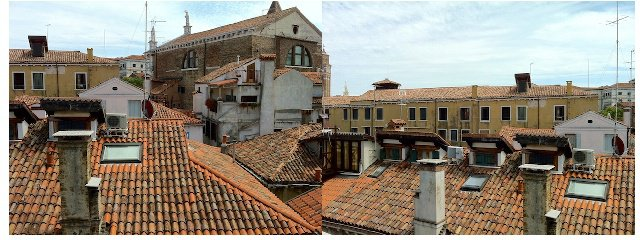
\includegraphics[width=\linewidth]{./Pictures/SIFT/siftMatching.jpg}
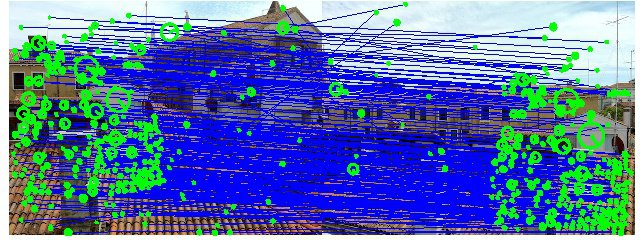
\includegraphics[width=\linewidth]{./Pictures/SIFT/siftMatchingDescriptor.jpg}
\caption{Use of SIFT Descriptor in matching }
\label{fig:siftMatching}
\end{figure}
\end{center}
%%%%%%%%%%%%%%%%
    Lazebnik et al. \cite{bagOfWords} gave an extension to normal BoW (Bag of Words model) by introducing Spatial Pyramid technique. In this technique, we create a spatial pyramid of an image by dividing the image in hierarchical spatial layers. Each division provides a finer sub-region and more spatial localized information about the image. We keep on dividing the image in layers and then calculate histogram over those 400 Visual words on these divisions.This approach works gives improved results on challenging scene recognition tasks as shown by Lazebnik et al. \cite{bagOfWords}. So considering this work, we also added Spatial Pyramid technique as defined in \cite{bagOfWords} .
    We did 2-level Spatial partitioning. In level 0, we have the full image, this gives 400 dimensional vector (the size of bag of visual words). In level 1, we partition the image in 4 sub regions, this gives $4 \times 400$ dimensional vector. In level 2, we have again partion each sub-region into 4 sub-regions, so we have $4 \times 4 =\  16 $ sub-regions. This gives us a $16 \times 400 $ dimensional descriptor. In this way, we have an image descriptor of size $8400$. We used the MATLAB implementation developed by \cite{bagOfWords} for computing the pyramid on the SIFT descriptors.
   A schematic diagram of  an image is shown in Figure \ref{fig:pyramidCompute}
%%%%%%%%%%%%%%%
 \begin{center}
\begin{figure}
\centering
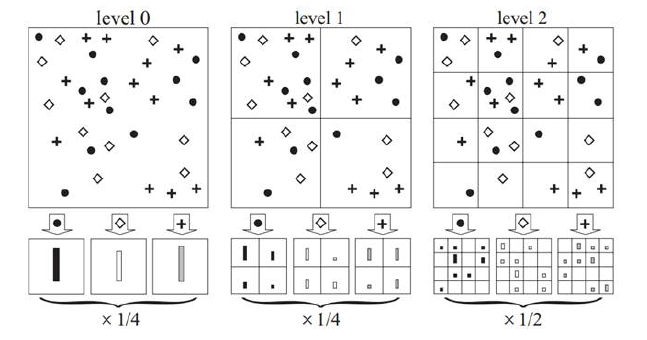
\includegraphics[width=\linewidth]{./Pictures/SIFT/pyramidCompute.jpg}
\caption{Computation of Spatial Pyramid over an image }
\label{fig:pyramidCompute}
\end{figure}
\end{center}
%%%%%%%%%%%%%%%%
    In figure \ref{fig:pyramidCompute}, we have represented the construction of the spatial pyramid. In this case, we have dictionary of three visual words represented by plus, circles and rhombus. The image is partitioned in 3 layers and for each layer in each sub-division, the count of each visual words is used to create the bin and then the spatial pyramid bins are weighted as given in \cite{bagOfWords}.
%%%%%%%%%%%%%%%%%%%%%%%%%%%%%%%%%
%%%%%%%%%%%%%%%%%%%%%%%%%%%%%%%%%
\subsection{GIST Features}
Just like SIFT features, GIST features also have their roots in the concept of primate vision. GIST features were first introduced by Aude Oliva and Antonio Torralba \cite{GIST} in 2001. They took the reference of Barrow, H.G. and Tannenbaum, J.M. 1978. paper \cite{barrow} which describes seminal vision in humans. Olivia and Torralba \cite{GIST} portrayed this seminal conception in computational vision. In case of scene recognition, human mind actually do progressive reconstruction of the input of local descriptors (edges, surfaces) integrated into complex decision layers. Therefore, the recognition of read word pictures may be initiated from some basic global descriptors, ignoring most of the details and object data.\\
  In \cite{GIST}, Olivia and Torralba suggested that recognition of real world pictures can be attempted with some small set of perceptual dimensions :  ruggedness, naturalness,roughness, expansion, openness.  This small set of perceptual dimension can be used as a way of recognizing a picture without going into tiresome process of segmentation and processing individual regions/objects. This low-dimesnional representation is termed as "Spatial Envelope" in \cite{GIST}. These Spatial Envelope Perceptual Dimension Descriptors can reliably computed using spectral and coarsely localized information.\\
   The model based on this spatial envelope generates a multidimensional space. In this projected space, scenes with semantically closed categories (e.g. sea, water, river, lake) are projected closely. The performance of this model emphasizes that for scene categorization and modeling a holistic representation of a scene, we do not need specific information about object shape or identity. This holistic representation is define as GIST of the scene.\\
  		Douze et al. \cite{douze} has shown that the GIST descriptor is very efficient and instrumental for web-scale search system for images. This indicates that GIST can also be an efficient feature for image classification. We, therefore, include GIST in our feature list.\\
  		We use the GIST implementation available on \cite{gistWebSite} as shown given by Olivia and Torralba \cite{GIST}. We first decompose the image using filters of 8 orientations for each of the 4 scales mentioned in \cite{GIST}.  This way we 32 oriented filter.
Then the image is represented as $4 \times 4 $ matrix. Output values of all filters are also normalized to $4 \times 4 $ matrix. THen the image is represented by the weighted combination of all these values representing into 8(orientation)$\times$ 4(scales) $\times$  4 $\times$ 4 (size of matrix) $=$ 512 dimensional vector.\\
		GIST can be easily extended for larger database because it is memory efficient and also computationally efficient. Even after being computationally efficient, It turns out to categorize natural images very well.
 %%%%%%%%%%%%%%%
\begin{center}
\begin{figure}	
\centering
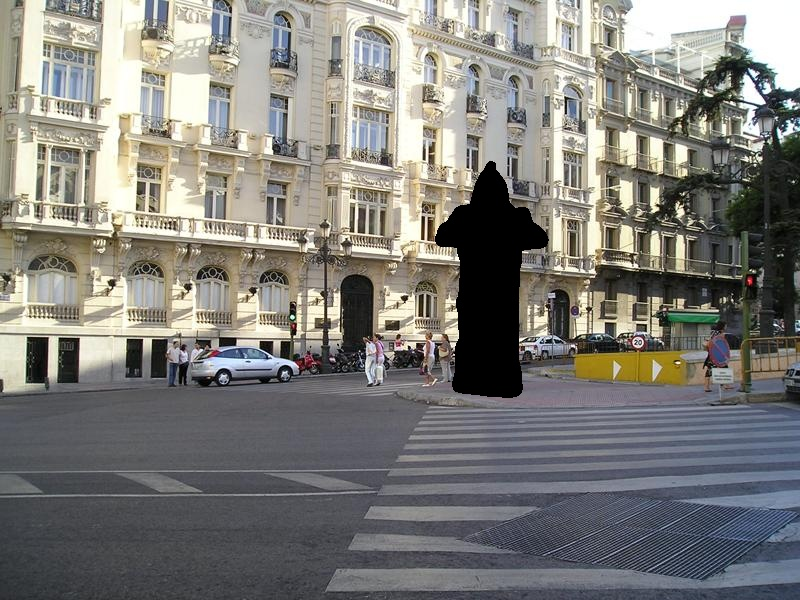
\includegraphics[width=4.5cm, height=4.5cm]{./Pictures/GIST/gistImage.jpg}
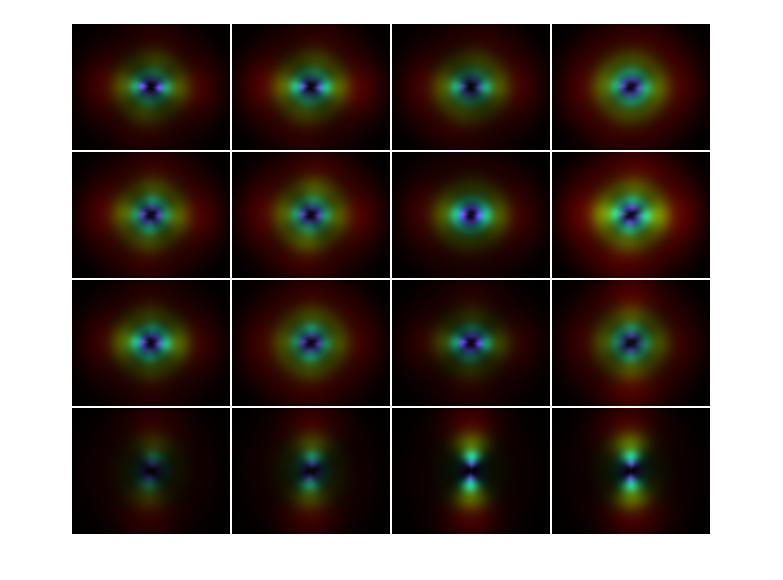
\includegraphics[width=4.5cm, height=4.5cm]{./Pictures/GIST/gistExample.jpg}
\caption{Example of GIST descriptors}
\label{fig:gistExample}
\end{figure}
\end{center}
%%%%%%%%%%%%%%%%  		
  		In Figure \ref{fig:gistExample}, we have shown GIST descriptors of an image. The left part is an image from our database and right is GIST descriptor for the image.
 %%%%%%%%%%%%%%%%%%%%%%%%%%%%%%%%%
 %%%%%%%%%%%%%%%%%%%%%%%%%%%%%%%%%
 %%%%%%%%%%%%%%%%%%%%%%%%%%%%%%%%%
\subsection{COLOR Space Features}
Colors for each pixel in an image can be represented using tuples of numbers, numbers can be three as in RGB model or four as in CMYK model). A color space is the way of such representation of colors, it is also called as color model or color system. Every color can be represented by a point in this color space. There are multiple color spaces, which are used to represent a color according to the application. Some of them are RGB , CMYK , HSV, CIELAB. In this section, we will give a brief overview of RGB and CIELAB, because we are using these for our thesis.

\subsubsection*{RGB Color Space}
RGB color space is consisted of three components Red, Green and Blue. Red, Green and Blue are considered as additive primary colors because these colors can be used to create a broad range of colors.\\ 
Colors can be created on computer monitors with color spaces based on the RGB color model, using the additive primary colors (red, green, and blue). In every pixel , we define the color using intensity values for each of these three colors. Yhe range of intensity value is 0-255. This leads to 16,777,216 different colors, when use different combinations of each of these colors. It is a reproduction medium dependent color space because it depicts different RGB values for the same image when computed on different devices, such as the phosphor (CRT monitor) or backlight (LCD monitor). RGB color space is been used in most of the modern display devices like Television, Computers, Mobile Phone displays etc.\\
\subsubsection*{CIELAB Color Space}
CIELAB Color Space describers all colors which are perceptibly visible for human beings. It was first introduced by the International Commission on Illumination in 2003. \cite{CIELAB}. It is also a three dimensional color space with three components of CIELAB are $L*$,$ a*$ and $b*$. $L*$ represents the lightness of color ranging from 0 to 100 in which 0 is black and 100 is white. $a*$ and $b*$ are color spaces. The range of both of these are -128 to +127. In this $a*$(+127) represent red color where as $a*$(-128) represents green color. $b*$(+127) represent yellow color where as $b*$(-128) represents blue color. \\
	To convert an image from CIELAB to RGB, we first convert the RGB image in CIEXYZ color space. Then we convert CIEXYZ to CIELAB. CIEXYZ is a color space introduced by CIE in 1931. For doing this we used MATLAB functions (makecform, applycform).
	Following are formula's for converting RGB color space to CIELAB. First conversion is from RGB to XYZ anf then we convert this into CIELAB. Conversion formula is mentioned below:
	Conversion from CIEXYZ space to CIELAB space:
		 $$ \left( \begin{array}{c} X \\ Y \\ Z \end{array} \right) =  \left( \begin{array}{ccc} 0.412453 & 0.357580 & 0.180423 \\ 0.212671 & 0.715160 & 0.072169 \\ 0.019334 & 0.119193 & 0.950227 \end{array} \right) \left( \begin{array}{c} R \\ B \\ G \end{array} \right)$$
		 \[
L^{*} =
  \begin{cases} 
      \hfill 116 \times (\frac{Y}{Y_n})^{({\frac{1}{3}})}    \hfill & \text{ if $(\frac{Y}{Y_n}) > 0.008856$ } \\
      \hfill 903.3 \times (\frac{Y}{Y_n}) \hfill & \text{otherwiise} \\
  \end{cases}
\]
 \[  a^* = 500 \times (f(\frac{X}{X_n})-f(\frac{Y}{Y_n})) \\ \]
   \[  b^* = 200 \times (f(\frac{Y}{Y_n})-f(\frac{Z}{Z_n}))\\ \]
 where,
  \[
  f(x)=
   \begin{cases} 
   \hfill x^{\frac{1}{3}} \hfill & \text{ if $( x > 0.008856)$ } \\
   \hfill 7.787 \times t + \frac{16}{116} \hfill & \text{,otherwise.} \\
   \end{cases}
  \]
 

	Here $X_n$, $Y_n$, and $Z_n$ are the tristimulus values of the reference white. 

\subsubsection*{Color Histogram}

Color Histogram is a very prominent feature in image classification problems. Color Histogram is a way to represent the cumulative distribution of colors in an image. It calculates the number of pixels lie in particular color range. The color ranges are histogram bins for the color histogram model. Color Histogram are independent to the rotational state of image. Therefore even if the image is tilted, it won't effect the classification. Apart from that computation efficiency is another strong reason behind using color histogram in classification problem. The disadvantage of color histogram is that it fails to capture the spatial distribution of the color in images and only captures the color information. \\
   As we described earlier in RGB color space subsection, RGB color space is dependent on the device., because of this device dependency,  RGB does not feel to be a right choice for our color histogram. Adding to that, CIELAB color space appears to be a better choice because of its perceptual uniformity and device in-dependency. Perceptual Uniformity means same quantity of perceptual effect is generated with same quantity of change in color values or we can say that visual effect is proportional to color values.\\
   We first used inbuilt MATLAB functions to convert the given images from RGB space to CIELAB color space. After that we  calculated the color histogram after dividing the image into 16 parts called blocks. Now we construct bins of 4 for each L,  a and b components. Thus we have totally 64 color bins. Thus for each block we get a 64 dimensional color histogram. When we combined the vectors we get a vector of $(16 \times 64 ) =1024$ dimensionality.
   
\subsection{Texture/ GLCM Feature Extraction}
 In order to extract some meaningful information from an image, it is important to get into human interpretable features. There are three types of such features which lead to perceptive interpretation of color images: spectral, textual and contextual features.\\
  In such human interpretable features, texture comes as an important feature. In normal terms we can define texture of an image as estimate of smoothness of that image. In everyday terms, texture can be defined with words as rough, bumpy, silky.\\
   A texture, which is rough, when touched has large difference between high and low points, with the distance between those points be very low. A smooth texture will usually has small difference between high and low points, with these points be distant.\\
   Image texture also works in the same. Except the high and low values, we have brightness values ( also referred as grey levels) instead of elevation. Instead of using hand or finger to judge the surface, a window or box is used to define the size of probe.\\
  GLCM or Gray Level Co-occurrence Matrix acts like a texture indicator for an image. This co-occurrence matrix represents the inter-pixel distance and spatial relationship between gray values over an image. This spatial interrelations of the grey tones actually determines the textural pattern.\\
  It was first introduced by Haralick et al \cite{haralick}, that's why it is also called as Haralick features . \\
  For calculating GLCM feature for an image, we first convert that image into a gray-scale one, because GLCM is actually an estimate of the occurrence of different combinations of pixels in a gray-scale image. The gray level co-occurrence matrix $G(i,j,\theta, d)$ can be as follows. The value of $G(i,j,\theta, d)$ is count of occurrences of the pair of pixels having gray value $i$ and $j$, where the distance between these pixels as $d$ and direction specified by angle $\theta$. In standard GLCM matrix, the angle are considered as 0\textdegree, 45\textdegree, 90\textdegree and 135\textdegree with $d=1\ pixel$. This directional component of $\theta$ makes it more powerful in a sense that it represent features from every angle of an image.\\
  %%%%%%%%%%%%%%%
 \begin{center}
\begin{figure}
\centering
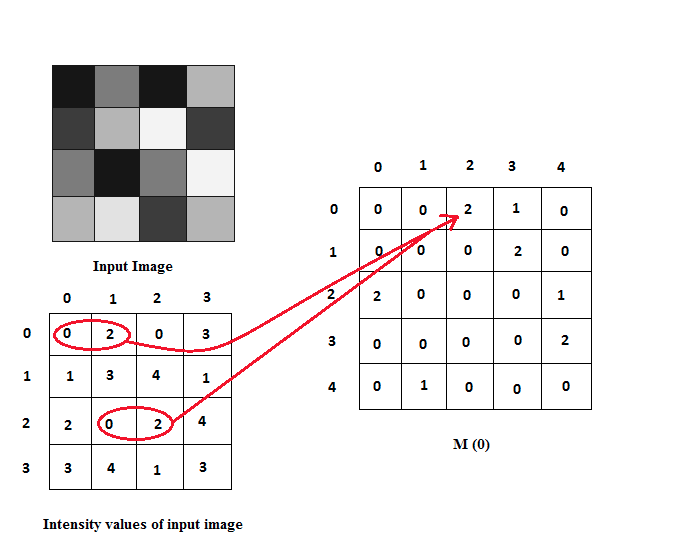
\includegraphics[width=\linewidth]{./Pictures/GLCM/process.jpg}
\caption{Co-occurence Matrix G(0\textdegree) generation for N=5 levels }
\label{fig:glcmMatrix}
\end{figure}
\end{center}
%%%%%%%%%%%%%%%%
 Figure \ref{fig:glcmMatrix} illustrate the process of finding co-occurrence matrices using $N=5$ levels. IT is showing gray-scale co-occurrence G(0\textdegree,$d=1$). We can observe that pixels (0,2) of the input is shown in G(0\textdegree,$d=1$) as 2 because we only have two occurrence of the pixel intensity value 0 with horizontally adjacent pixels with intensity = 2 in the input. We computed matrix G as symmetric, as we considered pair (0, 2) as (2, 0) as well. Matrix G can also be computed with non-symmetric measure.\\
    In our approach, we computed $G$ for all $\theta$ angles using $N=8$ with symmetry because increasing the gray levels further was decreasing the accuracy and lesser number of gray levels may not be sufficient enough to capture the texture adequately. We used MATLAB function to get this matrix. This step gives us four $8 \times 8$ matrices. As input is not re-sized to some predefined dimensions, we normalized each matrix for better comparison. After normalization, we got $1\times 64 $ dimensional vector for each matrix. We merge these to get $1\times 256 $ size vector for an image.
\subsection{HOG-LBP Features}
 HOG or Histogram of Oriented Gradients in one of the prominent used features for object recognition in Computer Vision. The idea behind this descriptor is that the object in an image can be shown by the some intensity gradients or distributed edge directions. HOG descriptor works in a localized region, therefore it does not get affected with illumination changes or geometric transformations like rotation, scale, or change in viewpoint. These descriptors were first used by Dalal and Triggs \cite{HOG} for human in 2005. After that these descriptors clubbed with LBP features are usually practiced for object recognition \cite{hog1}, \cite{hog2},\cite{hog3} etc. The steps of constructing HoG descriptors are shown in figure \ref{fig:hogProcess}.
%%%%%%%%%%%%%%%
 \begin{center}
\begin{figure}
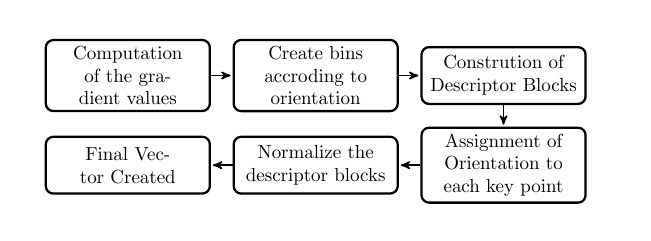
\includegraphics[width=\linewidth]{./Pictures/HOG/hogProcess.jpg}
\caption{Construction of HoG descriptors }
\label{fig:hogProcess}
\end{figure}
\end{center}
%%%%%%%%%%%%%%%%
Local Binary Pattern (LBP) is a texture classification feature first introduced by Ojala et al. \cite{ojala} in 1994. LBP captures the appearance of an image in a neighborhood of the pixel. A LBP is a string of bits, which contains one bit for each of the pixels in
the neighborhood. LBP does not get affected by monotonic gray level changes and acts as a good discriminator. Wang et al. \cite{wangHOG} tried combining HoG with LBP. The results indicated high improvement in performance in case of object detection. HoG looses its discriminating capability, if the image is cluttered with blurred edges. LBP acts as complementary to HoG in such cases. LBP uses uniform pattern to remove out the noisy edges from such cluttered image. In \cite{santana}, Santana et al. has also shown that the combination of HoG and LBP acts much better than the individual ones. We, therefore, consider combination of HoG and LBP for our classification. \\
We used VLFEAT \cite{vlfeat} library for computing HoG features. VLFEAT has two variants of HoG. One is UoCTTI variant, other is Dalal and Triggs's variant \cite{HOG}. We computed the UoCTTI variant HoG on each painting. This variant computes directed and also undirected gradients. Apart from this, it also has 4-dimensional texture-energy feature on a window size of $16 \time 16$ . We therefore obtain 31 dimensional HoG vector for each cell. \\
 For computing LBP features, we again used VLFEAT library \cite{vlfeat}.  VLFEAT considers $3*3$ neighborhood, this leads to LBP feature of 8 bit long string vector. This 8 bit long vector can assume $2^8 = 256$ possible values. These 256 possible values are further quantized into a smaller number of patterns. This uniform quantization makes LBP features computationally efficient. \\
 In this uniform quantization, we use following observations. There is one quantized pattern, for every bit, which has exactly one transition from 0 to 1 and one from 1 to 0 when scanned in anti-clockwise order. Plus one pattern comprising of two uniform LBPs and one pattern comprising all other LBPs. These observations yields total 58 patterns. When we concatenate both HoG and LBP vector descriptor we get combined vector of 89 dimension, Now we use bag of words approach on this combined HoG-LBP vector. We form a bag of 4000 visual words using the K-means and after that we combine the histogram on this visual dictionary for each vector, which gives a vector of 4000 dimension for each image.
%%%%%%%%%%%%%%%%
 \begin{center}
\begin{figure}
\centering
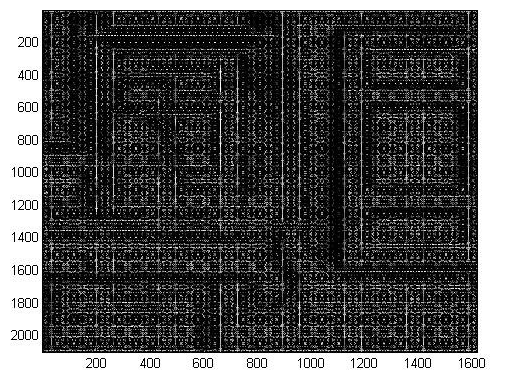
\includegraphics[width=4.5cm, height=4.5cm]{./Pictures/HOG/hogFeatures.jpg}
\caption{Example of HOG Descriptors}
\label{fig:hogExample}
\end{figure}
\end{center}
%%%%%%%%%%%%%%%%%
 In figure \ref{fig:hogExample}, we have  shown the HOG descriptor on an image. The left part is the original image and right part show the HoG descriptor for the image.
 


\section{Social Content Based Feature Extraction}
Social meta-data obtained from images has similar properties like text data-set, because we have tags, comments, groups all in normal language text. So, It makes sense to just only use the text processing methods here. But, this text data also has inherit structure of social network. We, therefore, to utilize this extra aspect, first construct node features over the social-metadata for each image as shown by \cite{Jure}. These node/social feature vectors have high dimensionality. We, therefore, use the topic modeling/text processing methods over these social features to construct a better and reduced representation. In \cite{tang}, Tang and Jie et al. have shown that such topic-level modeling of social-networking data leads to good result in finding patterns and inferences. These final low-dimensional features project the semantically close node features (like mountain, hill etc.) near to each other. We tried Latent Semantic Indexing(LSI), Latent Dirichlet allocation (LDA) and Random Projection (RP) methods for the purpose of dimesionality reduction and topic modeling. 
The process of constructing useful feature vectors out of the social meta-data obtained can be divided into following steps:\\
\begin{itemize}
\item Pre-analysis of Social Data
\item Constructing Node Features
\item Applying Topic Modeling/Text Processing Methods on Binary Social Features
\end{itemize} 
In the following part of this section, we will discuss each of these steps.
\subsection{Pre-analysis of Social Data}
   We first do preliminary observation about the tags and featured groups for image instances. The elementary observation suggests that tags are less structured are provided by any number of annotators and can include the information that is not easily detectable from content alone, such as location like sea-side or mountain ranges. Groups are similar to rags, with difference that the groups to which an image is featured, are chosen entirely by image's author.


\subsection{Constructing Node Features}
	There are some properties, which can be defined for a single image instances. eg. tags, groups etc. We call such features as node features, because these properties can be separately defined for each image/node. \\
	We first construct indicator vector encoding those words, groups and tags that appear in an image. For this , we first consider the 1000 most popular words, groups and tags across the entire data-set . As described in \cite{Jure}, this data set of only 1000 most popular words does not sufficiently represent the whole data. We, therefore, also consider any words, group and tags that our at least twice as frequently in images having the questioned label compared to the overall rate.  This way we will get the similar node features as described in \cite{Jure}. 
	 For developing this word feature, we utilize text from the image's title, it's comment thread, description after eliminating stop-words. This will give us more than 40000+ points. The node-feature vector is in a binary form and have high dimension. We have 0 and 1 as the value for each field in this vector corresponding the presence of word in the image data or not. We further convert this raw binary 0 and 1 form, in usable social features with the use of advance text processing methods like Latent Semantic Indexing and Random Projections.

\subsection{Applying Text Processing/Topic Modeling Methods on Binary Social Features}
 We, now, use dimensionality reduction cum text processing methods over these feature vectors. For text processing, we can consider each image as a document and the current node feature vector as a representation of dictionary. This vector represents the presence of a word in the document. Now, we have corpora of word features and in next step, we just need to use some topic modeling/text processing methods to get a feature vector with reduced dimension.
        We experimented with Latent Semantic Indexing, Random Projection and Latent Dirich-let Allocation as some possible methods to do such dimensionality reduction for sparse binary data.\\
\subsubsection{Latent Semantic Indexing}
Latent Semantic Indexing is actually a singular value decomposition method to identify patterns in the relationship among the semantic concepts in an unstructured collection of text. It is normally used for extraction of conceptual content of a body of text by establishing associations between those words which are show a similar contextual presence.\cite{Deerwester}
LSI is used in a variety of information retrieval and text processing applications which are increasingly used for electronic document discovery, publishing, government/intelligence community. \cite{e-discovery}
In typical information retrieval methods, an information retrieved by literally matching terms in search space with those of search query. However, this method, which purely depends on lexical matching, can be inaccurate. Since, there are many ways to express a given concept in real world, the literal matching may not provide us the relevant information. A better approach will be create a basis of conceptual topic for the search space. Latent Semantic Indexing tries to overcome the problems of lexical matching by using statistically derived conceptual indices instead of raw data. Latent Semantic Indexing  assumes that there is a hidden latent conceptual structure in raw features and which is not visible because of variability of word choices. A truncated SVD (Singular Value Decomposition ) is used to estimate this latent semantic structure. These statistically derived vectors proves to be more robust indicators of information than individual terms. 

\subsubsection{Basic Concept}
			Latent Semantic Indexing is a technique that projects the feature vectors into a space with "latent" semantic dimensions. In latent semantic space,  two feature vectors can have high cosine similarity even if they do not share any terms - as long as their terms are semantically similar in a sense to be described later. We can look at LSI as a
similarity metric that is an alternative to word overlap measures like tf.idf. 
		In terms of topic modeling and text processing, latent semantic indexing is the application of Singular Value Decomposition or SVD, to a "word-by-document" matrix. The projection into the latent semantic space is chosen such that the representations in the original space are changed as little as possible when measured by the sum of the squares of the
differences. 
		SVD represents a matrix $A$ as $\hat{A}$ in a lower dimensional space such that the "distance" between the two matrices (Which is measured by the 2-norm is minimized): \footnote{ The 2-norm for matrices is the equivalent of Euclidean distance for vectors.}
		$$ \delta = \| A - \hat{A} \| _{2}$$
		SVD project an n-dimensional space onto a k-dimensional space where $n \ll k$. Thus, the projection transforms a feature vector in n-dimensional word space into a vector in the k-dimensional reduced space. 
		We used GENSIM library \cite{gensim} in python for Latent Semantic Indexing of our data. It was developed by Radim Rehurek and Petr Sojka \cite{radimrehurek} for topic modeling with large corpora.
		 
\subsubsection{Latent Dirichlet allocation}
Latent Dirichlet allocation (LDA) is an another frequently used process in natural language processing. It is a generative model that allows set of observations to be depicted by unobserved groups explaining why some parts of the data are quite similar. For example in general natural language processing scenario, when the observations are words associated with a document, it tries computation to provide observations that each document is a mixture of a small number of topics and the each word's presence is dedicated to one of the document's concept. LDA was actually a graphical model presented in \cite{Blei} for topic discovery.
LDA has connection with image classification because in \cite{Li} a variation on LDA was used to automatically pit the natural images into categories, such as  forest and mountain, by assuming the images as words. 
	Latent Dirichlet allocation (LDA )uses generative probabilistic model of a corpus. The basic idea is that documents are represented as random mixtures over latent topics, where each topic is characterized by a distribution over words. There are many variants of LDA computation. In \cite{Blei}, LDA assumes the following generative process for each document $w$ in a corpus $D$:
	\begin{itemize}
	\item Choose $N \sim Poisson(\xi)$.
	\item Choose $\theta \sim Dir(\alpha)$.
	\item For each of the N words wn:
	\begin{itemize}
		\item  Choose a topic $z_n \sim Multinomial(\theta).$
		\item Choose a word $w_n$ from $p(w_n | z_n,\beta)$, a multi nomial probability conditioned on the topic $z_n$.
	\end{itemize}
	\end{itemize}
	%%%%%%%%%%%%%%%
 \begin{center}
\begin{figure}
\centering
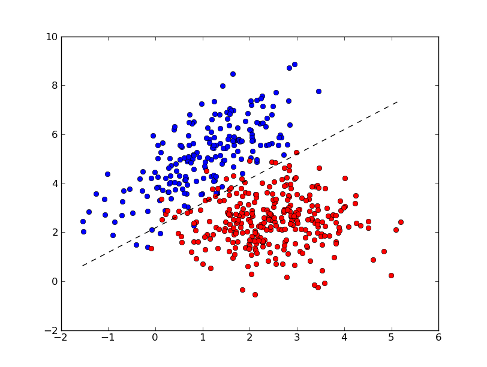
\includegraphics[width=\linewidth]{./Pictures/lda_binary.jpg}
\caption{Example of LDA in two-dimensional feature vector \cite{Blei}}
\label{fig:ldaExample}
\end{figure}
\end{center}
%%%%%%%%%%%%%%%%
	In figure \ref{fig:ldaExample}, we have shown an example of Linear Discriminant Analysis on a two-dimensional data set. The line in between discriminate the data set in two classes, where as the colors show the actual class labels.
	In our case the LDA does not provide a good results because we already have a textual data, which is oriented to solve a binary classification problem. This binary nature of topic leads to a too sparse feature generation from Latent Dirichlet allocation (LDA). This sparseness of features around images lead to low quality classification. LDA also fail if discriminatory information is
not in the mean but in the variance of the data  \cite{Blei}. We, therefore, discard this method for our computations.

\subsubsection{Random Projections}
Random Projections are a powerful methods for dimensionality reductions in application to image and text data. \cite{randproj}.  In \cite{rpCite}, Bingham introduced the random projections as a simpler and less erroneous dimensionality reduction tool for information retrieval from text and processing of images.  It is very instrumental in such case where reduction of the high dimensional data in a low dimension is essential, which if not reduced leads to heavy computation penalty without any significant gain. 
   Using random projection is significantly less expensive compared to techniques like principal component analysis. In random projection, the original high dimensional data is projected onto a lower dimensional subspace using a random matrix $R$. 
	In random projection, the original d-dimensional data is projected to a k-dimensional $(k << d)$ subspace through the origin, using a random $k \times d$ matrix $R$ whose columns have unit lengths. Using matrix notation where $X_{d\times N} $ is the original set of N d-dimensional observations,
$$ X^{RP}_{k\times N} = R_{k\times d} X_{d\times N} $$
is the projection of the data onto a lower k-dimensional subspace. The key idea of random mapping arises from the Johnson-Lindenstrauss lemma \cite{lemma}: if points in a vector space are projected onto a randomly selected subspace of suitably high dimension, then the distances between the points are approximately preserved.   
We write the Euclidean distance between two data vectors $x_1$ and $x_2$ in the original large-dimensional space as $\lVert x_1 - x_2 \rVert$. After the random projection, this distance is approximated by the scaled Euclidean distance of these vectors in the reduced space:
$$\sqrt{ d/k} \norm{R_{x_1} - R_{x_2}}$$
where d is the original and k the reduced dimensionality of the data set. The scaling term $\sqrt{d/k}$ takes into account the decrease in the dimensionality of the data: according to the Johnson-Lindenstrauss lemma \cite{lemma}.the expected norm of a projection of a unit vector onto a random subspace through the origin is $\sqrt{k/d}$
 The choice of the random matrix R is one of the key points of interest. The elements $r_{ij}$ of R are often Gaussian distributed,
but the Gaussian distribution can be replaced by a much simpler distribution such as
\[
	r_{ij} = \sqrt{3}*\begin{cases} 
	 +1 & \textrm{with proabibility $\frac{1}{6}$} \\
	 0 & \textrm{with proabibility $\frac{2}{3}$}\\
	-1 & \textrm{with proabibility $\frac{1}{6}$} \\
		\end{cases}
\]
   In fact, practically all zero mean, unit variance distributions of $r_ij$ would give a mapping that still satisfies the Johnson Lindenstrauss
lemma. This means further computational savings in feature computation, as the computations can be performed using integer arithmetic. Again for computing the random projections, we used the GENSIM library \cite{gensim} in python.  
	It has been found that even after being computationally light, Random projections is sufficiently accurate method for dimensionality reduction of high dimensional data \cite{Dasgupta}.
  


\subsection{Implementation of Dimensionality reduction}

Considering that we are using a large database and we need to do dimensionality reduction for such a data. We use an online version of aforementioned techniques. So that we don't have to bother about loading a whole data into memory space. \\
Both LSI and RP rely on TF-IDF ( term frequency - inverse document frequency ) as a fast pre processing step . \\
\cite{radimrehurek} gives a framework \cite{gensim} for doing all these text processing on large corpora in memory independent fashion. We use this as a tool to doing LSI and RP Compuation. On varying the number of dimension, in dimensionality reduction, we found that using 300 features in LSI and 400 features in RP gives us the best results.\\
In selecting the dimension the whole point is to reduce dimensionality in such a way that
we can go non-linear, which would be too costly and too susceptible to overtting with
thousands of binary features.
We directly convert the node features of dimension 40000+ in social features of dimension 300 (LSI) and dimension 400 (RP).  This conversion has been done in python using GENSIM and the converted file are in the LIBSVM format. \\

